\documentclass{article}
\usepackage[margin=1in]{geometry}
\usepackage{amsmath,amsthm,amssymb}
\usepackage{bbm,enumerate,mathtools}
\usepackage{tikz,pgfplots}
\usepackage{chessboard}
\usepackage[hidelinks]{hyperref}
\usepackage{multicol} % Problem 35

\newenvironment{question}{\begin{trivlist}\item[\textbf{Question.}]}{\end{trivlist}}
\newenvironment{note}{\begin{trivlist}\item[\textbf{Note.}]}{\end{trivlist}}
\newenvironment{references}{\begin{trivlist}\item[\textbf{References.}]}{\end{trivlist}}
\newenvironment{related}{\begin{trivlist}\item[\textbf{Related.}]\end{trivlist}\begin{enumerate}}{\end{enumerate}}


\begin{document}
  Starting with a configuration of coins, slide one coin at a time such that
  the coin ends up in a position where it is tangent to two other coins.
  \begin{figure}[ht!]
    \centering
    \begin{tikzpicture}[
      level distance=3cm,
      sibling distance = 4cm,
      level 1/.style={level distance=2.5cm},
      level 2/.style={level distance=3cm},
      level 4/.style={level distance=3.5cm}
    ]
      \node {
        \begin{tikzpicture}[scale=0.7]
          \foreach \x/\y/\n in {0/0/A, 1/0/B, 0/1/C, 1/1/D} {
            \draw[very thick] ({\x + \y/2}, {sqrt(3)/2 * \y}) circle (0.5) node {\n};
          }
        \end{tikzpicture}
      }
      child {
        node {
          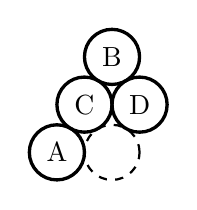
\begin{tikzpicture}[scale=0.7]
            \foreach \x/\y/\n in {0/0/A, 0/2/B, 0/1/C, 1/1/D} {
              \draw[very thick] ({\x + \y/2}, {sqrt(3)/2 * \y}) circle (0.5) node {\n};
            }
            \draw[thick, dashed] (1, 0) circle (0.5);
          \end{tikzpicture}
        }
        child {
          node {
            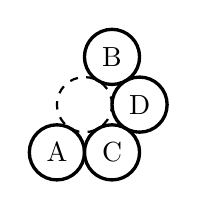
\begin{tikzpicture}[scale=0.7]
              \foreach \x/\y/\n in {0/0/A, 0/2/B, 1/0/C, 1/1/D} {
                \draw[very thick] ({\x + \y/2}, {sqrt(3)/2 * \y}) circle (0.5) node {\n};
              }
              \draw[thick, dashed] (0.5, {sqrt(3)/2}) circle (0.5);
            \end{tikzpicture}
          }
        }
        child {
          node {
            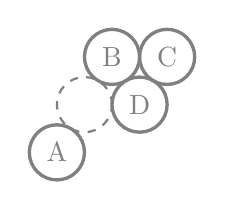
\begin{tikzpicture}[scale=0.7]
              \foreach \x/\y/\n in {0/0/A, 0/2/B, 1/2/C, 1/1/D} {
                \draw[gray, very thick] ({\x + \y/2}, {sqrt(3)/2 * \y}) circle (0.5) node {\n};
              }
              \draw[gray, thick, dashed] (0.5, {sqrt(3)/2}) circle (0.5);
            \end{tikzpicture}
          }
          child {
            node {
              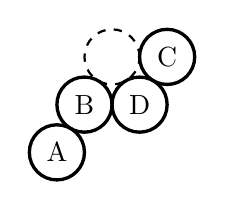
\begin{tikzpicture}[scale=0.7]
                \foreach \x/\y/\n in {0/0/A, 0/1/B, 1/2/C, 1/1/D} {
                  \draw[very thick] ({\x + \y/2}, {sqrt(3)/2 * \y}) circle (0.5) node {\n};
                }
                \draw[thick, dashed] (1, {sqrt(3)}) circle (0.5);
              \end{tikzpicture}
            }
          }
          child {
            node {
              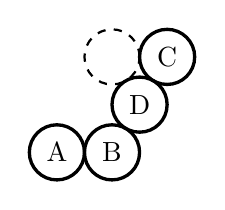
\begin{tikzpicture}[scale=0.7]
                \foreach \x/\y/\n in {0/0/A, 1/0/B, 1/2/C, 1/1/D} {
                  \draw[very thick] ({\x + \y/2}, {sqrt(3)/2 * \y}) circle (0.5) node {\n};
                }
                \draw[thick, dashed] (1, {sqrt(3)}) circle (0.5);
              \end{tikzpicture}
            }
          }
          child {
            node {
              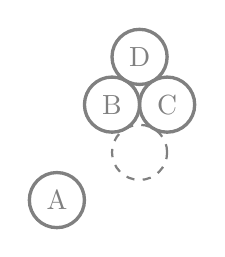
\begin{tikzpicture}[scale=0.7]
                \foreach \x/\y/\n in {0/0/A, 0/2/B, 1/2/C, 0/3/D} {
                  \draw[gray, very thick] ({\x + \y/2}, {sqrt(3)/2 * \y}) circle (0.5) node {\n};
                }
                \draw[gray, thick, dashed] (1.5, {sqrt(3)/2}) circle (0.5);
              \end{tikzpicture}
            }
            child {
              node {
                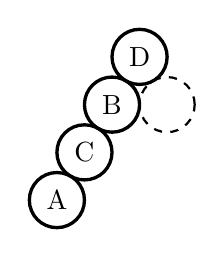
\begin{tikzpicture}[scale=0.7]
                  \foreach \x/\y/\n in {0/0/A, 0/2/B, 0/1/C, 0/3/D} {
                    \draw[very thick] ({\x + \y/2}, {sqrt(3)/2 * \y}) circle (0.5) node {\n};
                  }
                  \draw[thick, dashed] (2, {sqrt(3)}) circle (0.5);
                \end{tikzpicture}
              }
            }
          }
        }
      };
    \end{tikzpicture}

    \caption{
      All connected configurations of $4$ coins. Six out of the seven possible
      polyhexes are present.
    }
  \end{figure}
  \begin{question}
    In general, given $n$ coins starting in a ``spiral'' configuration, how many
    polyhexes can be reached by the above procedure?
  \end{question}

  \begin{related}
    \item What if this is done with hyperspheres in $\mathbb{R}^d$?
    \item Is there a sensible way to categorize non-connected configurations?
    \item Which polyhexes require the greatest amount of moves?
  \end{related}
  \begin{references}
    \item \url{https://en.wikipedia.org/wiki/Polyhex_(mathematics)}
  \end{references}
\end{document}
